\documentclass[11pt]{article}
\usepackage[a4paper,margin=1in]{geometry}
\usepackage[T1]{fontenc}
\usepackage[utf8]{inputenc}
\usepackage{lmodern,microtype}
\usepackage{amsmath,amssymb,amsthm,mathtools}
\usepackage{booktabs,array,float,placeins,enumitem}
\usepackage{graphicx,xcolor}
\usepackage{tikz}
\usetikzlibrary{arrows.meta,positioning,calc,decorations.pathreplacing}
\usepackage[numbers,super,sort&compress]{natbib}
\usepackage{caption}
\DeclareCaptionLabelSeparator{nhbbar}{ $|$ }
\captionsetup{labelfont=bf,labelsep=nhbbar,font=small}
\renewcommand{\figurename}{Supplementary Fig.}
\renewcommand{\tablename}{Supplementary Table}
\usepackage{setspace}
\usepackage{hyperref}
\hypersetup{colorlinks=true,citecolor=blue,linkcolor=blue,urlcolor=blue}
\setstretch{1.08}
\raggedbottom
\graphicspath{{figures/}}

\newtheorem{proposition}{Proposition}[section]
\newtheorem{lemma}{Lemma}[section]
\newtheorem{corollary}{Corollary}[section]
\newtheorem{definition}{Definition}[section]
\newtheorem{remark}{Remark}[section]
\newcommand{\E}{\mathbb{E}}
\newcommand{\Prob}{\mathbb{P}}
\newcommand{\1}{\mathbf{1}}
\newcommand{\Astar}{A^{*}}
\newcommand{\prov}[1]{\par\vspace{1pt}{\footnotesize\color{black!60}\textsf{\textbf{Verification:} #1}}\par\vspace{2pt}}
\renewcommand{\thesection}{S\arabic{section}}
\renewcommand{\theequation}{S\arabic{equation}}
\definecolor{verm}{HTML}{D55E00}
\definecolor{blu}{HTML}{0072B2}

\title{\bfseries Supplementary Information\\[1mm] \large When losing delegitimizes the game: cognitive dissonance turns collective failure into self-defending error}
\author{Gabriel Bontemps \and Abhishek Banerjee}
\date{\today}

\begin{document}
\maketitle
\tableofcontents

\subsection*{Verification status: how to read this document}
Every numbered statement below carries a \textsf{Verification} line built from four tags.
\textsf{Lean-certified (T$n$)}: the named algebraic identity or equivalence is
machine-checked in Lean~4 (Section~\ref{s:lean} lists statements, files, hashes and axiom
closures); the tag covers exactly the named algebraic step, never the surrounding
analysis. \textsf{Proved here}: a complete proof appears in this document.
\textsf{Imported}: the step is taken from the cited source; each such citation was
verified against an authoritative bibliographic record before use, and theorem or chapter
numbers internal to a source are cited only where independently confirmed (the
verification log ships in the replication bundle). \textsf{Numerical (frozen record)}:
the statement is established by simulation under a frozen design, and the named record in
the bundle is its evidence. Results we consider non-standard are flagged as such where
they appear.

\section{Notation and full model specification}
\label{s:model}

\subsection{Entities and state}
Time is discrete, $t\in\mathbb N_0$ (one bandit trial per step). Agents $i\in V=\{1,\dots,N\}$ are partitioned into two equal communities $V_1,V_2$ ($N_c=N/2$); $c(i)$ denotes $i$'s community. Arms $a\in\{1,2\}$ pay Bernoulli rewards with means $\mu_1>\mu_2$; write $\Delta\mu=\mu_1-\mu_2$ and $a^\star=1$. Community coupling is the row-stochastic matrix
\begin{equation}
B=\begin{pmatrix}1-\Gamma & \Gamma\\ \Gamma & 1-\Gamma\end{pmatrix},
\end{equation}
inducing balanced block weights $W_{ij}=B_{c(i)c(j)}/N_{c(j)}$. Each agent carries action values $Q_{i,t}(a)\in[0,1]$, legitimacy $L_{i,t}\in[0,1]$, and aspiration $A_{i,t}\in[0,1]$. Supplementary Table~\ref{tab:notation} collects all symbols.

\begin{table}[H]\centering\small
\caption{Notation.}
\label{tab:notation}
\begin{tabular}{llp{8.6cm}}
\toprule
Symbol & Range & Meaning \\
\midrule
$Q_{i,t}(a)$ & $[0,1]$ & latent action value \\
$L_{i,t}$ & $[0,1]$ & legitimacy: evidential weight granted to the reward rule \\
$A_{i,t}$ & $[0,1]$ & aspiration / entitlement benchmark \\
$C_{i,t}$ & $[0,1)$ & decisiveness, $|2\Prob_{i,t}(a{=}1)-1|$ \\
$S_{i,t}(a)$ & $[0,1]$ & anticipatory credibility field \\
$\lambda,\eta$ & $\ge0$ & anticipatory / retrospective social gains \\
$\beta,\sigma,a_{\mathrm{thr}}$ & & quantal-choice parameters; $\kappa_\beta:=2\beta a_{\mathrm{thr}}/\sigma^2=12$ at defaults \\
$\alpha$ & $(0,1)$ & private learning rate \\
$\delta_{i,t}$ & $[-1,1]$ & private prediction error $R-Q(a_t)$ \\
$\Delta^F_{i,t}$ & $[-1,1]$ & entitlement discrepancy $R-A$ \\
$D^F_{i,t}$ & $\ge0$ & asymmetric discomfort, equation~\eqref{eq:DF} \\
$\phi^-,\phi^+$ & $\phi^->\phi^+\ge0$ & disadvantageous / advantageous discomfort weights \\
$\tau^F$ & $\ge0$ & acceptability (tolerance) threshold \\
$X_t,K_t$ & & excess $[D^F-\tau^F]_+$; acceptability $\1\{D^F\le\tau^F\}$ \\
$\nu_F,\nu_R$ & $\ge0$ & legitimacy loss / repair rates ($>0$ for the gated agent; $0$ in the gate-off control) \\
$\rho,\chi$ & $[0,1]$ & aspiration adaptation rate; social anchoring weight \\
$\bar R^{\mathrm{ref}}_{i,t}$ & $[0,1]$ & reference outcome (exposure-weighted or population mean) \\
$\Gamma$ & $[0,\tfrac12]$ & cross-community permeability \\
$\Astar(\mu)$ & & critical aspiration, equation~\eqref{eq:astar} \\
$\rho_c$ & & critical adaptation rate, equation~\eqref{eq:rhoc} \\
\bottomrule
\end{tabular}
\end{table}

\subsection{Within-trial schedule}
Supplementary Fig.~\ref{fig:schedule} fixes the schedule; all prediction errors, the discomfort, and the gate use \emph{pre-update} states, and all updates are applied synchronously.

\begin{enumerate}[leftmargin=1.8em,itemsep=0pt]
\item \textbf{Field.} $\phi_{c,t-1}(a)=N_c^{-1}\sum_{j\in V_c}\1\{a_{j,t-1}=a\}C_{j,t-1}$ and $S_{i,t}(a)=\sum_d B_{c(i)d}\,\phi_{d,t-1}(a)$; $S_{i,0}\equiv0$.
\item \textbf{Choice.} $V_{i,t}(a)=Q_{i,t}(a)+\lambda S_{i,t}(a)$; $\Delta_{i,t}=V_{i,t}(1)-V_{i,t}(2)$; $\Prob(a_{i,t}{=}1)=\Lambda(\kappa_\beta\Delta_{i,t})$ with $\Lambda(x)=(1+e^{-x})^{-1}$; decisiveness $C_{i,t}=|2\Prob(a_{i,t}{=}1)-1|$.
\item \textbf{Outcome.} $R_{i,t}\sim\mathrm{Bern}(\mu_{a_{i,t}})$, independent across $(i,t)$ given actions.
\item \textbf{Observables.} Community statistics $\bar R_{c,t}$ (mean reward), $w_{c,t}(a)=N_c^{-1}\sum_{j\in c}\1\{a_{j,t}=a\}C_{j,t}$ and $u_{c,t}(a)=N_c^{-1}\sum_{j\in c}\1\{a_{j,t}=a\}C_{j,t}R_{j,t}$; exposures $e_{i,t}(a)=\sum_d B_{c(i)d}w_{d,t}(a)$, $o_{i,t}(a)=\sum_d B_{c(i)d}u_{d,t}(a)$.
\item \textbf{Conflicts (pre-update states).} $\delta_{i,t}=R_{i,t}-Q_{i,t}(a_{i,t})$; social error $\mathrm{soc}_{i,t}(a)=o_{i,t}(a)-e_{i,t}(a)Q_{i,t}(a)$; discomfort
\begin{equation}
D^F_{i,t}=\phi^-[A_{i,t}-R_{i,t}]_+ +\phi^+[R_{i,t}-A_{i,t}]_+ .
\label{eq:DF}
\end{equation}
\item \textbf{Synchronous updates.} With gate $g_{i,t}$ ($=L_{i,t}$; $\equiv1$ for the ungated control; $=\pi_{i,t}$ for the Bayesian rival):
\begin{align}
Q_{i,t+1}(a) &= \Pi_{[0,1]}\Big(Q_{i,t}(a)+\alpha\,g_{i,t}\,\delta_{i,t}\1\{a=a_{i,t}\}+\eta\,g_{i,t}\,\mathrm{soc}_{i,t}(a)\Big),\label{eq:Qfull}\\
L_{i,t+1} &= \Pi_{[0,1]}\Big(L_{i,t}-\nu_F[D^F_{i,t}-\tau^F]_+ +\nu_R\1\{D^F_{i,t}\le\tau^F\}\Big),\label{eq:Lfull}\\
A_{i,t+1} &= \Pi_{[0,1]}\Big((1-\rho)A_{i,t}+\rho\big[(1-\chi)R_{i,t}+\chi\bar R^{\mathrm{ref}}_{i,t}\big]\Big),\label{eq:Afull}
\end{align}
with $\bar R^{\mathrm{ref}}_{i,t}=\sum_d B_{c(i)d}\bar R_{d,t}$ (local) or $N^{-1}\sum_j R_{j,t}$ (global visibility).
\end{enumerate}

\begin{figure}[H]
\centering
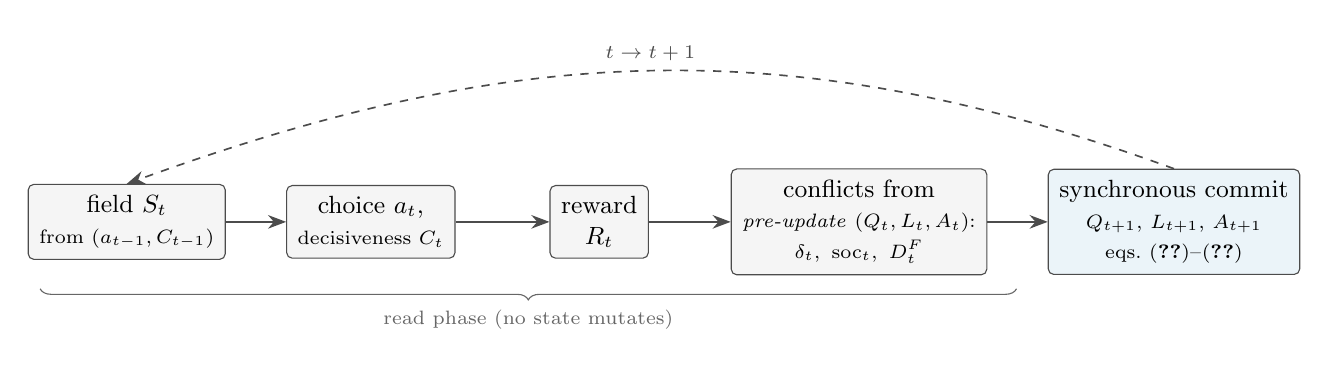
\begin{tikzpicture}[font=\small,
  st/.style={draw=black!70, rounded corners=2pt, align=center, inner sep=4pt, minimum height=7.5mm},
  pre/.style={st, fill=black!4},
  upd/.style={st, fill=blu!8},
  arr/.style={-{Stealth[length=2.3mm]}, semithick, black!70}]
\node[pre] (f) at (0,0) {field $S_t$\\ \scriptsize from $(a_{t-1},C_{t-1})$};
\node[pre] (ch) at (3.1,0) {choice $a_t$,\\ \scriptsize decisiveness $C_t$};
\node[pre] (r) at (6.0,0) {reward\\ $R_t$};
\node[pre] (pe) at (9.3,0) {conflicts from\\ \scriptsize \emph{pre-update} $(Q_t,L_t,A_t)$:\\ \scriptsize $\delta_t,\ \mathrm{soc}_t,\ D^F_t$};
\node[upd] (up) at (13.3,0) {synchronous commit\\ \scriptsize $Q_{t+1},\,L_{t+1},\,A_{t+1}$\\ \scriptsize eqs.~\eqref{eq:Qfull}--\eqref{eq:Afull}};
\draw[arr] (f)--(ch); \draw[arr] (ch)--(r); \draw[arr] (r)--(pe); \draw[arr] (pe)--(up);
\draw[arr, dashed] (up.north) to[out=160,in=20] node[above,font=\scriptsize]{$t\to t+1$} (f.north);
\draw[decorate,decoration={brace,mirror,amplitude=4pt}, black!60]
  (-1.1,-0.85) -- node[below=4pt,font=\scriptsize]{read phase (no state mutates)} (11.3,-0.85);
\end{tikzpicture}
\caption{\textbf{Within-trial schedule.} All conflicts are computed from pre-update states and all three state variables commit simultaneously, eliminating order artefacts between private, social, and frame revision. The field $S_t$ carries one trial of delay (it is built from $t-1$ actions and decisiveness).}
\label{fig:schedule}
\end{figure}

\section{The dissonance functional and the derivation of the updates}
\label{s:derivation}

\begin{definition}[Per-period dissonance]
Given the trial data $(a_t,R_t)$ and the aspiration $A_t$,
\begin{equation}
\mathcal D(Q,L)=\frac{L}{2}\big(R_t-Q(a_t)\big)^2+w_f\Big[L\,X_t+(1-L)\,\kappa\,K_t\Big],
\qquad X_t=[D^F_t-\tau^F]_+,\ K_t=\1\{D^F_t\le\tau^F\}.
\label{eq:D}
\end{equation}
\end{definition}
The evidence term is Festinger-weighted: a reward--belief discrepancy is dissonant in proportion to the legitimacy granted to the rule that produced the reward. The frame term prices both directions of frame--experience conflict: legitimacy under intolerable deprivation ($LX$), and grievance under acceptable outcomes ($(1-L)\kappa K$).

\begin{proposition}[Margin-wise gradients]
\label{p:grad}
(i) $\partial\mathcal D/\partial Q(a_t)=-L\,(R_t-Q(a_t))$, so a gradient step of gain $\alpha$ on the belief margin is $Q\mapsto Q+\alpha L\delta$. The expansion is exactly quadratic:
\begin{equation}
\tfrac{L}{2}(R-(Q+h))^2-\tfrac{L}{2}(R-Q)^2=-L(R-Q)h+\tfrac{L}{2}h^2
\label{eq:T1}
\end{equation}
(machine-checked as T1), so the linear response is the entire first-order content. (ii) The frame margin is affine in $L$ with slope $w_f(X_t-\kappa K_t)$; a gradient step of gain $\nu$ gives $L\mapsto L-\nu_F X_t+\nu_R K_t$ with $\nu_F=\nu w_f$ and $\nu_R=\nu w_f\kappa$, i.e.\ equation~\eqref{eq:Lfull}. (iii) With $\nu=0$, $L_0=1$, equation~\eqref{eq:Qfull} is the Robbins--Monro recursion whose only rest points on visited arms satisfy $Q^\star(a)=\E[R\,|\,a]=\mu_a$; the induced choice is the quantal response to the true means.
\end{proposition}
\prov{(i) Lean-certified (T1); (ii), (iii) proved here; the contraction step in (iii) is Lean-certified (T5a).}
\begin{proof}
Write $\delta=R_t-Q(a_t)$. (i) For a perturbation $h$ of the chosen-action value, the
displayed expansion~\eqref{eq:T1} is an exact identity with no remainder beyond the
quadratic term (T1); hence $\partial\mathcal D/\partial Q(a_t)=-L\delta$, and a gradient
step of gain $\alpha$ is $Q\mapsto Q+\alpha L\delta$, which is equation~\eqref{eq:Qfull}
restricted to the private channel.

(ii) The frame margin differentiates the frame term only (the lexicographic convention;
Remark~\ref{r:nonlex} drops it): $\partial_L\,w_f[LX_t+(1-L)\kappa K_t]
=w_f(X_t-\kappa K_t)$, which is constant in $L$. The gradient step of gain $\nu$ is
therefore $L\mapsto L-\nu w_f X_t+\nu w_f\kappa K_t$; the stated reparameterization and
the projection $\Pi_{[0,1]}$ give equation~\eqref{eq:Lfull} exactly. Because $X_t K_t=0$
by construction, loss and repair never fire on the same trial.

(iii) At $\nu=0$ the gate is frozen at $L_0=1$ and the visited-arm recursion is
$Q'=Q+\alpha(R-Q)$. Conditioning on the arm, $\E[Q'-\mu_a\,|\,Q]=(1-\alpha)(Q-\mu_a)$:
the conditional mean contracts geometrically (the identity is T5a at $L=1$, iterated by
T5b), so the unique rest point of the conditional mean on any arm visited infinitely
often is $Q^\star(a)=\mu_a$, and the induced stationary choice probability is
$\Lambda\big(\kappa_\beta[\mu_1-\mu_2+\lambda(S(1)-S(2))]\big)$---the quantal response to
the true means at the prevailing field.
\end{proof}

\begin{remark}[The non-lexicographic variant]
\label{r:nonlex}
If the frame margin is differentiated through the evidence term as well, the legitimacy update gains $-\nu\,\delta_t^2/2$: surprise itself erodes legitimacy. Since $\E[\delta^2]\le\tfrac14+\mathrm{bias}^2\le1$, the extra term is a bounded state-dependent erosion that renames constants in every threshold statement below ($\tau^F\mapsto\tau^F_{\mathrm{eff}}$, $\nu_R\mapsto\nu_R-\nu\E[\delta^2\,|\,K{=}1]/2$); the region structure and sign characterizations are unchanged. The lexicographic form is used throughout the main text; the variant's distinctive prediction (legitimacy erosion in fair-but-noisy environments) is left untested here.
\end{remark}

\begin{remark}[Myopia]
The agent takes one proximal step per margin per period. A forward-looking dissonance manager would trade current frame comfort against future material payoffs; nothing here speaks to that problem.
\end{remark}

\section{Drift analysis and the critical aspiration}
\label{s:drift}

\begin{lemma}[Four-region drift decomposition]
\label{l:regions}
Fix an arm with mean $\mu$ and condition on aspiration $A$, with $L$ away from the clip
boundaries. With Bernoulli outcomes the discomfort takes exactly two values: on failure
(probability $1-\mu$), $D^F=\phi^-A$; on success, $D^F=\phi^+(1-A)$. The $(A,\tau^F)$
plane splits into four regions (Supplementary Fig.~\ref{fig:regions}):
\begin{align}
\E[\Delta L]=
\begin{cases}
\nu_R & \text{(R0)}\\[2pt]
-\nu_F(1-\mu)(\phi^-A-\tau^F)+\nu_R\,\mu & \text{(R1)}\\[2pt]
-\nu_F\,\mu(\phi^+(1-A)-\tau^F)+\nu_R(1-\mu) & \text{(R2)}\\[2pt]
-\nu_F\big[(1-\mu)(\phi^-A-\tau^F)+\mu(\phi^+(1-A)-\tau^F)\big] & \text{(R3)}
\end{cases}
\label{eq:regions}
\end{align}
with R0: $A\le\tau^F\!/\phi^-$ and $\phi^+(1-A)\le\tau^F$ (nothing binds); R1: $A>\tau^F\!/\phi^-$, success acceptable (generic); R2: failure acceptable but $\phi^+(1-A)>\tau^F$ (windfall); R3: both bind.
\end{lemma}
\prov{Proved here.}
\begin{proof}
From equation~\eqref{eq:DF}, failure ($R=0$) gives $D^F=\phi^-A$ and success ($R=1$)
gives $D^F=\phi^+(1-A)$; no other values occur. Away from the clips, equation
\eqref{eq:Lfull} gives $\Delta L=-\nu_F[D^F-\tau^F]_+ +\nu_R\1\{D^F\le\tau^F\}$, so
\begin{equation*}
\E[\Delta L]=(1-\mu)\big(-\nu_F[\phi^-A-\tau^F]_+ +\nu_R\1\{\phi^-A\le\tau^F\}\big)
+\mu\big(-\nu_F[\phi^+(1-A)-\tau^F]_+ +\nu_R\1\{\phi^+(1-A)\le\tau^F\}\big).
\end{equation*}
Each branch is piecewise linear with one switch; crossing the two indicator conditions
yields the four sign patterns, and substituting each pattern gives the four displayed
rows. Each region's expression is affine in $A$, which is what makes the subsequent sign
analysis exact.
\end{proof}

R2/R3 require $\phi^+(1-A)>\tau^F$, i.e.\ tolerance below the advantageous discomfort of success. Over the admissible range these regions are empty exactly when the inequality fails at the R0/R2 boundary $A=\tau^F/\phi^-$, i.e.\ when $\phi^+(1-\tau^F/\phi^-)\le\tau^F$; rearranging gives the standing restriction $\phi^+\le\tau^F\big/\big(1-\tau^F/\phi^-\big)$ under which the headline analysis proceeds (at defaults: $0.25\le 0.3/0.7\approx0.43$, satisfied with slack). We report the excluded corner as the \emph{windfall-delegitimation corner}.

\begin{proposition}[Critical aspiration]
\label{p:astar}
In R1, $\E[\Delta L]>0\iff \nu_F(1-\mu)\phi^-A<\nu_F(1-\mu)\tau^F+\nu_R\mu \iff A<\Astar(\mu)$ with
\begin{equation}
\Astar(\mu)=\frac{\tau^F+(\nu_R/\nu_F)\,\mu/(1-\mu)}{\phi^-}.
\label{eq:astar}
\end{equation}
The cleared-form equivalence, the divided form, and the branch-weighted expectation form are machine-checked (T2, T2b, T4; Section~\ref{s:lean}).
\end{proposition}
\prov{Lean-certified end-to-end in R1: T4 (branch-weighted expectation $\iff$ cleared inequality) chained with T2 (cleared $\iff$ sign) and T2b (cleared $\iff A<\Astar$ under the positivity hypotheses $\nu_F>0$, $\phi^->0$, $0<\mu<1$). The one-line rearrangement below is the human-readable shadow of that chain.}
\begin{proof}
In R1, $\E[\Delta L]=-\nu_F(1-\mu)(\phi^-A-\tau^F)+\nu_R\mu$ by Lemma~\ref{l:regions}.
Positivity follows from clearing: $\E[\Delta L]>0\iff\nu_F(1-\mu)\phi^-A
<\nu_F(1-\mu)\tau^F+\nu_R\mu$ (T2/T4), and dividing by $\nu_F(1-\mu)\phi^->0$ gives
$A<\Astar(\mu)$ with $\Astar$ as displayed (T2b).
\end{proof}

$\Astar$ is increasing in $\mu$: better arms are easier to forgive. At default parameters ($\tau^F=0.3$, $\nu_R/\nu_F=0.25$, $\phi^-=1$): $\Astar(0.4)=0.3+0.25\cdot\tfrac{0.4}{0.6}=0.3+\tfrac16=\tfrac{7}{15}\approx0.467$ and $\Astar(0.6)=0.3+0.25\cdot\tfrac{0.6}{0.4}=0.675$.

\begin{figure}[H]
\centering
\resizebox{.96\textwidth}{!}{%
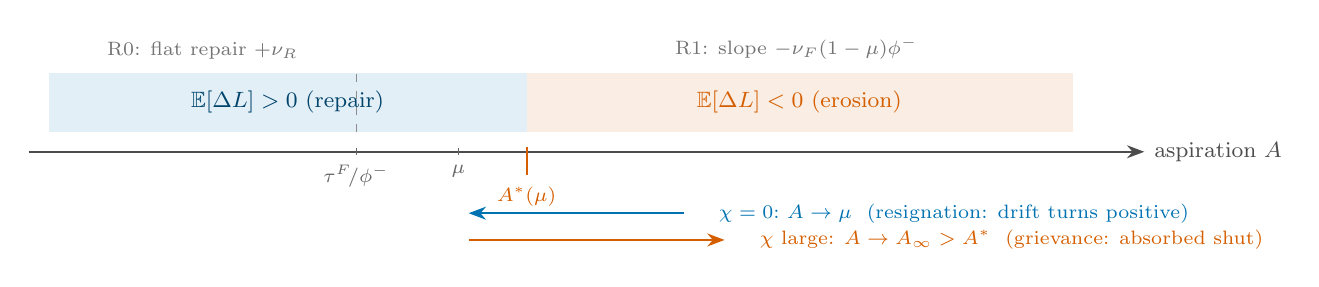
\begin{tikzpicture}[font=\small, xscale=13, yscale=1.0,
  arr/.style={-{Stealth[length=2.2mm]}, semithick, black!70}]
% sign bands
\fill[blu!11]  (0,0.25) rectangle (0.4667,1.0);
\fill[verm!11] (0.4667,0.25) rectangle (1.0,1.0);
\node[font=\footnotesize, text=blu!60!black]  at (0.233,0.63) {$\E[\Delta L]>0$ (repair)};
\node[font=\footnotesize, text=verm] at (0.733,0.63) {$\E[\Delta L]<0$ (erosion)};
\draw[black!45, dashed] (0.3,0.25) -- (0.3,1.0);
\node[font=\scriptsize, text=black!55, anchor=south] at (0.15,1.05) {R0: flat repair $+\nu_R$};
\node[font=\scriptsize, text=black!55, anchor=south] at (0.73,1.05) {R1: slope $-\nu_F(1-\mu)\phi^-$};
% axis with staggered tick labels
\draw[arr] (-0.02,0) -- (1.07,0) node[right, font=\footnotesize, black!70]{aspiration $A$};
\draw[black!60] (0.3,0.045) -- (0.3,-0.045) node[below, font=\scriptsize]{$\tau^F\!/\phi^-$};
\draw[black!60] (0.4,0.045) -- (0.4,-0.045) node[below, font=\scriptsize]{$\mu$};
\draw[verm, semithick] (0.4667,0.055) -- (0.4667,-0.30);
\node[font=\scriptsize, text=verm, anchor=north] at (0.4667,-0.32) {$\Astar(\mu)$};
% aspiration dynamics, staggered rows below the axis
\draw[arr, blu] (0.62,-0.78) -- (0.41,-0.78);
\node[font=\scriptsize, text=blu, anchor=west] at (0.645,-0.78)
  {$\chi=0$:\ $A\to\mu$\ \ (resignation: drift turns positive)};
\draw[arr, verm] (0.41,-1.12) -- (0.66,-1.12);
\node[font=\scriptsize, text=verm, anchor=west] at (0.685,-1.12)
  {$\chi$ large: $A\to A_\infty>\Astar$\ \ (grievance: absorbed shut)};
\end{tikzpicture}}%

\caption{\textbf{Drift regions on an arm of mean $\mu=0.4$} (generic restriction R2/R3 excluded). Legitimacy repairs below $\Astar$ and erodes above it; the aspiration dynamics (equation~\eqref{eq:Afull}) move $A$ towards $\mu$ (resignation, blue) or towards $(1-\chi)\mu+\chi\mu_{\mathrm{ref}}$ (grievance, vermilion), which is what decides the long run.}
\label{fig:regions}
\end{figure}

\section{Resignation, relative deprivation, and the race}
\label{s:theorems}

\subsection{Resignation}
\begin{proposition}[Self-extinguishing grievance, $\chi=0$]
\label{p:resign}
Let outcomes be i.i.d.\ Bernoulli($\mu$) and $\chi=0$. Then (i) $\E[A_t]=\mu+(A_0-\mu)(1-\rho)^t$ and $\mathrm{Var}(A_\infty)=\rho\,\mu(1-\mu)/(2-\rho)$, so $A_t$ concentrates in an $O(\sqrt\rho)$ band around $\mu$; (ii) if $\mu<\Astar(\mu)$, there is $t^\ast<\infty$ with $\E[\Delta L_t]>0$ for all $t>t^\ast$, and $L_t$ (reflected at 1) returns to a neighbourhood of 1; (iii) the trapped dwell decomposes as
\begin{equation}
T_{\mathrm{dwell}}\;\approx\;\underbrace{\tfrac1\rho\ln\tfrac{A_0-\mu}{\Astar-\mu}}_{\text{aspiration adaptation}}\;+\;\underbrace{T_{\mathrm{repair}}(\nu_R)}_{\text{gate reopening}}\;+\;\underbrace{O\!\big(\tfrac1{\alpha \bar L}\big)}_{\text{relearning}} .
\end{equation}
\end{proposition}
\prov{Proved here; the concentration step imports Hoeffding's inequality\cite{BLM2013} and the return step imports drift-to-hitting-time bounds\cite{Hajek1982}; the relearning identity in (iii) is Lean-certified (T5a, T5b).}
\begin{proof}
(i) The mean is the standard AR(1) computation; for the variance,
$\mathrm{Var}(A_{t+1})=(1-\rho)^2\mathrm{Var}(A_t)+\rho^2\mu(1-\mu)$, whose fixed point is
$\rho^2\mu(1-\mu)/(1-(1-\rho)^2)=\rho\,\mu(1-\mu)/(2-\rho)$. For the band, write
$A_t-\E[A_t]=\rho\sum_{k=0}^{t-1}(1-\rho)^{t-1-k}(R_k-\mu)$, a weighted sum of independent
centred variables bounded in $[-\mu,1-\mu]$ with squared weight norm
$\rho^2\sum_{k<t}(1-\rho)^{2k}\le\rho/(2-\rho)$. Hoeffding's inequality for weighted sums of
bounded independent variables\cite{BLM2013} gives
$\Prob\big(|A_t-\E A_t|\ge\varepsilon\big)\le2\exp\!\big(-\tfrac{(2-\rho)\varepsilon^2}{2\rho}\big)$,
i.e.\ a sub-Gaussian band of width $O(\sqrt\rho)$ at every $t$, uniformly.

(ii) Fix $\varepsilon\in(0,\Astar-\mu)$ and let $t^\ast_\varepsilon$ be the (deterministic-mean)
time at which $\E[A_t]=\Astar-2\varepsilon$; by (i), for $t>t^\ast_\varepsilon$ the event
$\{A_t<\Astar-\varepsilon\}$ fails with probability at most $2e^{-c\varepsilon^2/\rho}$ per
period. On that event the conditional drift of $L_t$ is bounded below: in R1,
$\E[\Delta L_t\mid\mathcal F_t]=\nu_F(1-\mu)\phi^-(\Astar-A_t)\ge\nu_F(1-\mu)\phi^-\varepsilon
=:\varepsilon_0>0$ (and $=\nu_R>0$ in R0), while $|\Delta L_t|\le\nu_F\phi^-+\nu_R$ always.
A bounded-increment process on $[0,1]$ (reflected at 1) whose drift is bounded below by
$\varepsilon_0$ off the target set is exactly the setting of Hajek's drift
analysis\cite{Hajek1982}: the first-passage time of $L_t$ into any neighbourhood
$[1-\eta,1]$ has finite mean $O(1/\varepsilon_0)$ and exponential tails, and the subsequent
occupation of sets bounded away from 1 is exponentially rare. The reflection itself is
benign for this import: off the target set $[1-\eta,1]$ the projection at $1$ never acts,
so increments and drift there are those of the unprojected recursion, and where the
projection does act it moves $L_t$ monotonically towards (never past) the target set, so
it can only shorten the first passage and tighten the occupation bound. Intersecting with the
sub-Gaussian aspiration band and a union bound over periods gives the return statement.

(iii) The relearning scale follows from the machine-checked gated contraction (T5a/T5b):
with step gain $\alpha L$, $Q'-\mu=(1-\alpha L)(Q-\mu)$, so overturning a value gap of size
$G$ costs $\sim\ln(G/\varepsilon)/(\alpha\bar L)$ visited trials and diverges as $\bar L\to0$.
The condition $\mu<\Astar(\mu)$ rearranges to $\phi^-\mu-\tau^F<(\nu_R/\nu_F)\mu/(1-\mu)$;
its failure is the \emph{absolute-deprivation corner}, in which even fully adapted poverty
remains intolerable.
\end{proof}

\subsection{Relative deprivation}
\begin{proposition}[Persistence requires visible unequal success]
\label{p:reldep}
With anchoring $\chi>0$ to a reference stream of mean $\mu_{\mathrm{ref}}$, $A_\infty=(1-\chi)\mu+\chi\mu_{\mathrm{ref}}$ in mean, and the gate is absorbed shut iff
\begin{equation}
\chi(\mu_{\mathrm{ref}}-\mu)>\Astar(\mu)-\mu .
\label{eq:reldep}
\end{equation}
Under exposure-weighted (local) reference with polarized communities, $\mu_{\mathrm{ref}}-\mu=\Gamma\,\Delta\mu$, so the effective condition is $\chi\Gamma\Delta\mu>\Astar-\mu$: comparison that rides the influence ties is first-order weak. Under global visibility, $\mu_{\mathrm{ref}}$ is the population mean and the condition decouples from $\Gamma$.
\end{proposition}
\prov{Proved here (absorption as a hitting-and-occupation statement, importing ref.~\citenum{Hajek1982}; concentration as in Proposition~\ref{p:resign}); the equilibrium caveat below is numerical (frozen $(\rho,\chi)$ mapping record, \texttt{pt2.csv}).}
\begin{proof}
\emph{Limit aspiration.} Taking expectations in equation~\eqref{eq:Afull} with own-arm
mean $\mu$ and reference-stream mean $\mu_{\mathrm{ref}}$,
$\E[A_{t+1}]=(1-\rho)\E[A_t]+\rho[(1-\chi)\mu+\chi\mu_{\mathrm{ref}}]$, an AR(1) recursion
with unique fixed point $A_\infty=(1-\chi)\mu+\chi\mu_{\mathrm{ref}}$ approached
geometrically at rate $\rho$. The driving noise $(1-\chi)(R_t-\mu)+\chi(\bar
R^{\mathrm{ref}}_t-\mu_{\mathrm{ref}})$ is bounded in $[-1,1]$, so the weighted-sum
concentration argument of Proposition~\ref{p:resign}(i) applies verbatim and $A_t$
concentrates in an $O(\sqrt\rho)$ band around its mean (an averaged reference stream only
shrinks the bound).

\emph{Absorption, $\Leftarrow$.} Suppose $\chi(\mu_{\mathrm{ref}}-\mu)>\Astar-\mu+\varepsilon$
for some $\varepsilon>0$, i.e.\ $A_\infty>\Astar+\varepsilon$. After the mean-crossing
time, $\{A_t>\Astar+\varepsilon/2\}$ fails with per-period probability at most
$2e^{-c\varepsilon^2/\rho}$, and on that event Lemma~\ref{l:regions} bounds the drift
above: $\E[\Delta L_t\mid\mathcal F_t]\le-\nu_F(1-\mu)\phi^-\varepsilon/2=:-\varepsilon_0$
in R1, with increments bounded by $\nu_F\phi^-+\nu_R$. The drift criterion of
ref.~\citenum{Hajek1982} then gives a finite-mean, exponential-tail first passage of
$L_t$ into any neighbourhood $[0,\eta)$ of the floor and exponentially small long-run
occupation of sets bounded away from it. ``Absorbed shut'' is this occupation statement:
excursions above any level $\eta>0$ have exponentially small frequency, matching the
simulated gate's behaviour at the trap.

\emph{Absorption, $\Rightarrow$ (contrapositive).} If
$\chi(\mu_{\mathrm{ref}}-\mu)<\Astar-\mu$ then $A_\infty<\Astar$, and
Proposition~\ref{p:resign}(ii) applies with $\mu$ replaced by the mixture mean: the
drift of $L$ is eventually bounded below by a positive constant, so $L$ returns to a
neighbourhood of 1 and occupation of low-$L$ sets is exponentially rare---the gate is not
absorbed. The knife-edge $A_\infty=\Astar$ is excluded as non-generic.

\emph{Local versus global reference.} Under exposure weighting with polarized
communities (community $c$ concentrated on its own arm), the reference of a member of
the losing community is $\bar R^{\mathrm{ref}}=(1-\Gamma)\mu+\Gamma(\mu+\Delta\mu)$ in
mean, so $\mu_{\mathrm{ref}}-\mu=\Gamma\Delta\mu$; substituting gives the displayed
condition. Under global visibility $\mu_{\mathrm{ref}}$ is the population mean,
independent of $\Gamma$.
\end{proof}
\emph{Equilibrium caveat (established by the mapping runs).} Equation~\eqref{eq:reldep} treats $\mu_{\mathrm{ref}}$ as fixed. When the reference population itself corrects, $\mu_{\mathrm{ref}}$ rises with everyone's outcomes and the condition must be evaluated at the \emph{equilibrium} reference; this is why fast-adaptation persistence predicted from static $\chi_c$ failed in the regime maps, and why persistence is confined to the slow-$\rho$ band.

\begin{corollary}[Relative deprivation at the corrected reference]
\label{c:reldepeq}
Let $\mu_{\mathrm{ref}}^{\mathrm{eq}}$ be the reference earning after the reference population has corrected. Permanent closure requires $\chi\big(\mu_{\mathrm{ref}}^{\mathrm{eq}}-\mu\big)>\Astar(\mu)-\mu$ at the \emph{equilibrium} reference; the same inequality verified at a pre-correction reference is necessary but not sufficient. In particular, if correction lifts the whole population to a common earning ($\mu_{\mathrm{ref}}^{\mathrm{eq}}=\mu$), the left side vanishes and no anchoring weight $\chi$ sustains closure---the content of the refuted static-$\chi_c$ prediction.
\end{corollary}
\prov{Immediate from Proposition~\ref{p:reldep} read at the equilibrium reference; the empirical location of the persistence band is numerical (frozen record \texttt{pt2.csv}).}

\subsection{The race condition}
\begin{proposition}[Critical adaptation rate]
\label{p:race}
In the deterministic continuous-time mean field on the inferior arm with $\chi=0$, $A(t)=\mu_2+(A_0-\mu_2)e^{-\rho t}$ and $\dot L=-\nu_F(1-\mu_2)\phi^-\big(A(t)-\Astar\big)$ while in R1. Integrating to the drift-reversal time $t^\ast=\rho^{-1}\ln\frac{A_0-\mu_2}{\Astar-\mu_2}$,
\begin{equation}
L(t^\ast)=L_0-\frac{\nu_F(1-\mu_2)\phi^-}{\rho}\Big[(A_0-\Astar)-(\Astar-\mu_2)\ln\tfrac{A_0-\mu_2}{\Astar-\mu_2}\Big],
\end{equation}
so $L$ is absorbed at the floor before the drift reverses iff $\rho<\rho_c$ with
\begin{equation}
\rho_c=\frac{\nu_F(1-\mu_2)\phi^-}{L_0}\Big[(A_0-\Astar)-(\Astar-\mu_2)\ln\tfrac{A_0-\mu_2}{\Astar-\mu_2}\Big].
\label{eq:rhoc}
\end{equation}
The bracket is positive whenever $A_0>\Astar$ (strict convexity of $x\mapsto x-\ln x$) and vanishes as $A_0\downarrow\Astar$.
\end{proposition}
\prov{Proved here (the displayed integration is the proof); the reading of $\rho_c$ as the small-gain limit of the stochastic system imports constant-stepsize and finite-population approximation theorems (paragraph below); the placement of the empirical boundary is numerical (frozen record \texttt{pt2.csv}).}
\begin{proof}
$A(t)$ solves $\dot A=\rho(\mu_2-A)$ from $A_0$, giving the displayed exponential, and
$A(t^\ast)=\Astar$ defines $t^\ast$. While in R1, Lemma~\ref{l:regions} gives $\dot
L=-\nu_F(1-\mu_2)\phi^-(A(t)-\Astar)$; substituting $A(t)-\Astar
=(A_0-\mu_2)e^{-\rho t}-(\Astar-\mu_2)$ and integrating from $0$ to $t^\ast$,
\begin{equation*}
L(t^\ast)=L_0-\nu_F(1-\mu_2)\phi^-\Big[\tfrac{A_0-\mu_2}{\rho}\big(1-e^{-\rho t^\ast}\big)-(\Astar-\mu_2)\,t^\ast\Big],
\end{equation*}
and using $e^{-\rho t^\ast}=(\Astar-\mu_2)/(A_0-\mu_2)$ collapses the bracket to the
displayed form. Absorption before drift reversal is $L(t^\ast)\le0$, which rearranges to
$\rho\le\rho_c$ as stated. At the frozen defaults with $A_0=0.8$:
$\Astar(0.4)=7/15$, so the bracket is
$(0.8-\tfrac{7}{15})-(\tfrac{7}{15}-0.4)\ln\tfrac{0.8-0.4}{7/15-0.4}
=\tfrac13-\tfrac1{15}\ln6\approx0.3333-0.1195=0.2138$, and
$\rho_c=0.05\cdot0.6\cdot1\cdot0.2138/1=0.00641$.
\end{proof}
The dense $(\rho,\chi)$ map places the finite-size empirical boundary just below $\rho_c$ (horizon censoring: persistence is measured at $T=600$; finite-$N$ escape events).

\emph{Direct test of the absorption threshold.} Persistence-to-horizon is a dwell-time observable and therefore an indirect check on $\rho_c$, which governs \emph{absorption}. A frozen single-agent experiment isolates the absorption event itself: fixed-rate $\mathrm{Bern}(\mu_2)$ outcomes, $A_0=0.8$, $\chi=0$, defaults otherwise, outcome defined as $L$ reaching the floor before $A$ crosses $\Astar(\mu_2)$ (400 runs per point, 15 log-spaced $\rho$ values, horizon cap $5000$ trials, zero censored runs). The absorption probability falls from $1.000$ at $\rho\le4.6\times10^{-3}$ to $0.000$ at $\rho\ge8.8\times10^{-3}$ across a sharp sigmoid whose midpoint sits at $\rho=0.0068$, $6\%$ above the closed-form $\rho_c=0.00641$ (Supplementary Fig.~\ref{fig:scaling}f). The two finite-gain corrections therefore go in opposite directions for the two observables, and both are small: realized absorption extends slightly \emph{above} $\rho_c$ (outcome fluctuations let $L$ reach the floor on paths whose mean avoids it), while population persistence at a fixed horizon ends slightly \emph{below} it (horizon censoring and finite-$N$ escapes).

\paragraph{Validity of the deterministic computation.} The pair $(A_t,L_t)$ is a
constant-gain stochastic-approximation process with gains $(\rho,\nu_F)$ and bounded
increments. Two standard results license reading the ODE threshold $\rho_c$ as the
small-gain limit of the stochastic system. First, for constant gains the piecewise-linear
interpolation of the iterates converges weakly, as the gains tend to zero with their ratio
fixed, to the solution of the stated mean ODE on any finite horizon of order one in rescaled
time; this is the constant-stepsize theory of stochastic
approximation\cite{KushnerYin2003,Borkar2008} (Chapter~9 of the latter), and the race is
decided on exactly such a horizon, $t^\ast=O(1/\rho)$. Second, at the population level the
community averages over $N$ agents track the same drift field with fluctuations that vanish
exponentially in $N$ on finite horizons, by the deterministic-approximation theorem for
stochastic evolution in finite populations\cite{BenaimWeibull2003}. Neither result covers
the kinks of the drift field at the region boundaries of Section~\ref{s:drift} or the
reflection at $L\in\{0,1\}$ globally; both are benign here because the race path crosses
each boundary transversally and finitely often. The expected finite-gain corrections are a
boundary displaced slightly \emph{below} $\rho_c$ (early absorption by fluctuation, horizon
censoring at $T=600$, finite-$N$ escapes), which is what the dense $(\rho,\chi)$ map shows.


\section{Mean-field reduction of the network model}
\label{s:meanfield}

Write $m_{c,t}$ for community-$c$ mass on arm 1, $\bar Q_{c,t}(a)$, $\bar L_{c,t}$, $\bar A_{c,t}$ for community means, and $S_{c,t}(a)=\sum_d B_{cd}\phi_{d,t-1}(a)$ for the field, with $\phi_{c,t}(a)\approx C_{c,t}(a)\,m^{(a)}_{c,t}$, $m^{(1)}=m$, $m^{(2)}=1-m$. The reduction consists of three elementary but load-bearing computations.

\begin{lemma}[Deterministic choice map]
\label{l:choicemap}
In the homogeneous deterministic limit (all members of a community share $(Q,L,A)$), the
community's arm-1 mass is the exact logistic
\begin{equation}
m_{c,t}=\Lambda\!\Big(\kappa_\beta\big[\bar Q_{c,t}(1)-\bar Q_{c,t}(2)+\lambda(S_{c,t}(1)-S_{c,t}(2))\big]\Big).
\end{equation}
\end{lemma}
\prov{Proved here.}
\begin{proof}
Each member holds the same augmented values $V(a)=\bar Q(a)+\lambda S(a)$, so each
chooses arm 1 independently with the same probability
$\Lambda(\kappa_\beta[V(1)-V(2)])$; the community mass is that probability exactly in
the deterministic (law-of-large-numbers) limit, and the expression is exact---no
linearization of $\Lambda$ is involved. Heterogeneity within a community makes
\eqref{l:choicemap} the first-order term of a mixture; the mapping runs quantify the
residual.
\end{proof}

\begin{lemma}[Gated contraction of community values]
\label{l:contraction}
On a visited arm, the community-mean value recursion contracts towards the arm mean at
modulus $1-(\alpha+\eta e)\bar L$, where $e$ is the exposure weight of the retrospective
channel on that arm.
\end{lemma}
\prov{The one-channel identity is Lean-certified (T5a; $n$-step form T5b); the two-channel combination is proved here.}
\begin{proof}
Both channels in equation~\eqref{eq:Qfull} move $Q$ towards an unbiased estimate of the
arm mean: conditioning on the arm, $\E[\delta]=\mu_a-\bar Q(a)$ for the private channel,
and the retrospective target $o(a)/e(a)$ is a decisiveness-weighted average of Bernoulli
outcomes on the same arm, also of mean $\mu_a$. Taking conditional means,
$\bar Q'(a)-\mu_a=\big(1-(\alpha+\eta e)\bar L\big)(\bar Q(a)-\mu_a)$, the T5a identity
with step gain $(\alpha+\eta e)\bar L$; iterating gives the geometric $n$-step form
(T5b). The modulus degrades to 1 as $\bar L\to0$: a closed gate freezes the community's
values at whatever error they carry.
\end{proof}

\begin{lemma}[Between-community gap decay]
\label{l:gap}
Any quantity mixed linearly through the coupling $B$ with mixing weight $\psi$ (the
benchmark under local reference, for instance) satisfies
\begin{equation}
z_{1,t+1}-z_{2,t+1}=(1-2\psi\Gamma)(z_{1,t}-z_{2,t}),
\end{equation}
i.e.\ geometric decay of the gap at rate $2\psi\Gamma$.
\end{lemma}
\prov{Lean-certified (T3).}
\begin{proof}
With $z_{c}'=(1-\psi)z_c+\psi[(1-\Gamma)z_c+\Gamma z_{-c}]$, subtracting the two
community equations cancels the common terms and leaves the displayed recursion; T3
certifies the induction to the $t$-step geometric form.
\end{proof}

Two consequences used in the text. (i) \emph{Lock-in self-consistency}: by
Lemma~\ref{l:choicemap}, a wrong-consensus rest point ($m\approx0$) requires the field
advantage to dominate the value deficit, $\lambda[S(2)-S(1)]>\bar Q(1)-\bar Q(2)$, with
$\bar Q(2)\to\mu_2$ by Lemma~\ref{l:contraction} and decisiveness near 1 at a locked
point; this is the transmission condition that the $(A_0,\lambda)$ boundary traces.
(ii) \emph{Slow--fast structure}: for $\rho\ll\nu_F,\alpha$ the aspiration is the slow
variable dragging the fast $(m,\bar Q,\bar L)$ layer across the $\Astar$ boundary, the
configuration treated by two-timescale stochastic approximation\cite{Borkar2008}
(Chapter~6): the fast layer tracks the quasi-static attractor indexed by the current
$A$; the trap is entry of that attractor into the $L$-absorbed branch before $A$
crosses back---which is exactly Proposition~\ref{p:race} lifted to the network, and why
$\rho_c$ computed from the single-community field predicts the network boundary's
scale.
\prov{(i), (ii): consequences of the lemmas above at the stated level of rigour; their quantitative accuracy is numerical (frozen mapping records \texttt{pt1.csv}, \texttt{pt2.csv}, \texttt{pt4.csv}).}

\section{Stochastic-approximation connections and open mathematics}
\label{s:sa}

Equation~\eqref{eq:Qfull} at fixed gate is a constant-step Robbins--Monro scheme; its ODE limit is $\dot Q(a)=L(\mu_a-Q(a))$ on visited arms, with the gated Bellman operator a contraction of modulus $1-\alpha L$ (T5a) and geometric $n$-step decay (T5b). The standard machinery goes a long way here, and we use it rather than reprove it: constant-gain interpolations converge weakly to the mean ODE on finite rescaled horizons\cite{KushnerYin2003,Borkar2008}; the interpolated process is an asymptotic pseudotrajectory of the limiting semiflow, so its accumulation points are constrained to the flow's chain-recurrent set\cite{Benaim1999}; finite-population averages admit exponential deterministic-approximation bounds on finite horizons\cite{BenaimWeibull2003}; drift conditions with bounded increments convert the sign results of Section~\ref{s:drift} into hitting- and occupation-time bounds\cite{Hajek1982}; and the slow--fast decomposition at $\rho\ll\nu_F$ is the two-timescale configuration\cite{Borkar2008}. The coupled system retains two genuinely non-standard features that these results do not cover globally: the step size $L_t$ is itself a state variable driven by a reflected, threshold-censored recursion \eqref{eq:Lfull}, and the drift field is only piecewise smooth across the R0--R3 regions of Section~\ref{s:drift} (a stochastic recursive inclusion in the sense of Chapter~5 of ref.~\citenum{Borkar2008} at the kinks). We therefore claim convergence and absorption results only at the levels established: deterministic mean field (closed forms above), algebraic identities (machine-checked), finite-horizon tracking (cited above), and finite-size behaviour (simulation with frozen designs and distributional cross-validation). \textbf{Not proved here}: almost-sure statements for the coupled $(Q,L,A)$ chain under constant gains beyond finite horizons; fluid limits for the network with decisiveness-weighted fields; metastable escape asymptotics for the locked phase. These are stated as open so the record cannot be misread as claiming them.

\section{Machine-checked statements}
\label{s:lean}

Seven theorems compile under official Lean~4 v4.28.0, core library only, over $\mathbb Q$ (the rational parameter space used in all experiments); axiom closure of every declaration is exactly \{\texttt{propext}, \texttt{Classical.choice}, \texttt{Quot.sound}\}, with no \texttt{sorry}. File hashes and full logs ship in the bundle, and the sources with their verification records are published in the authors' repositories (directory \texttt{formal\_diss/}, branch \texttt{lean-diss-core}).

\begin{center}\small
\begin{tabular}{llp{8.0cm}}
\toprule
ID & File & Statement (informal) \\
\midrule
T1 & \texttt{DissCore.lean} & exact quadratic expansion \eqref{eq:T1} behind Proposition~\ref{p:grad}(i) \\
T2 & \texttt{DissCore.lean} & drift sign $\iff$ cleared inequality (no hypotheses needed) \\
T2b & \texttt{DissCore.lean} & cleared inequality $\iff A<\Astar$ under positivity hypotheses \\
T3 & \texttt{DissCore.lean} & gap recursion $\Rightarrow$ geometric decay $(1-2\psi\Gamma)^t$ \\
T4 & \texttt{DissBridge.lean} & branch-weighted $\E[\Delta L]>0 \iff$ cleared inequality (R1) \\
T5a & \texttt{DissBridge.lean} & gated contraction $Q'-m=(1-\alpha L)(Q-m)$ \\
T5b & \texttt{DissBridge.lean} & $n$-step geometric form of T5a \\
\bottomrule
\end{tabular}
\end{center}

\noindent Chaining T4$\to$T2$\to$T2b certifies $\E[\Delta L]>0\iff A<\Astar$ in R1 end-to-end. Scope: algebra only; nothing stochastic, network-level, or behavioural is certified.

\section{The Bayesian rival: specification and the self-confirming trap}
\label{s:rival}

The rival holds $H_{\mathrm{fair}}$ (arms pay learnable means, plug-in $\hat\mu_a=Q(a)$ clipped to $[0.05,0.95]$) against $H_{\mathrm{rig}}$ (both arms pay Bernoulli $\mu_{\mathrm{rig}}=0.4$). Log-odds $\ell_{i,t}=\ln\frac{\pi_{i,t}}{1-\pi_{i,t}}$ update on the own outcome and on exposure-weighted observed outcomes,
\begin{equation}
\ell_{t+1}=\mathrm{clip}_{[-12,12]}\Big(\ell_t+\underbrace{R\ln\tfrac{\hat\mu_{a}}{\mu_{\mathrm{rig}}}+(1-R)\ln\tfrac{1-\hat\mu_{a}}{1-\mu_{\mathrm{rig}}}}_{\text{own}}+\underbrace{\textstyle\sum_a e(a)\big[\bar r(a)\ln\tfrac{\hat\mu_a}{\mu_{\mathrm{rig}}}+(1-\bar r(a))\ln\tfrac{1-\hat\mu_a}{1-\mu_{\mathrm{rig}}}\big]}_{\text{observed}}\Big),
\end{equation}
learning proceeds at $\alpha\pi_t$, and choice uses the model-averaged contrast $\pi_t(Q(1)-Q(2))$.

\begin{lemma}[Self-confirming trap as a KL identity]
\label{l:kl}
Let the community's realized outcome stream have mean $\mu_2$ and let the fair model
hold any plug-in estimate $\hat\mu\in(0,1)$. The per-trial expected log-likelihood-ratio
increment in favour of $H_{\mathrm{fair}}$ is
\begin{equation}
g(\hat\mu)\;=\;\mu_2\ln\tfrac{\hat\mu}{\mu_{\mathrm{rig}}}+(1-\mu_2)\ln\tfrac{1-\hat\mu}{1-\mu_{\mathrm{rig}}}
\;=\;\mathrm{KL}\big(\mathrm{Bern}(\mu_2)\,\|\,\mathrm{Bern}(\mu_{\mathrm{rig}})\big)-\mathrm{KL}\big(\mathrm{Bern}(\mu_2)\,\|\,\mathrm{Bern}(\hat\mu)\big).
\end{equation}
If $\mu_2=\mu_{\mathrm{rig}}$ (a wrong consensus on the arm whose mean the rigged
hypothesis asserts), then $g(\hat\mu)=-\mathrm{KL}\big(\mathrm{Bern}(\mu_{\mathrm{rig}})\|\mathrm{Bern}(\hat\mu)\big)\le0$,
with equality only at $\hat\mu=\mu_{\mathrm{rig}}$: no fair-model estimate can generate
expected evidence for fairness.
\end{lemma}
\prov{Proved here (the identity is two lines of algebra); the resulting population-level freeze and its dissolution by permeability are numerical (frozen records \texttt{results\_experiments.json}, \texttt{pt3.csv}).}
\begin{proof}
Add and subtract $\mu_2\ln\mu_2+(1-\mu_2)\ln(1-\mu_2)$ in $g(\hat\mu)$ and collect terms
into the two Kullback--Leibler divergences displayed. The second statement is
non-negativity of KL with its equality case.
\end{proof}

\paragraph{The group-contingent variant (added in response to the coarseness concern).}
A rival whose rigged hypothesis is about \emph{us}---``the rule pays our choices at
$\mu_{\mathrm{rig}}$ regardless; it asserts nothing about others''---receives zero
log-likelihood contribution from observed others (their outcomes have the same law under
both hypotheses), so visible success elsewhere neither defeats nor confirms the
hypothesis. Implemented in the network (identical grid and seed structure as the
permeability sweep): under isolation it traps like the global variant ($m_2=0.00$,
trust $0.10$ at $\Gamma=0$); under permeability it heals---but through its own outcomes:
the still-open prior lets the social channel correct behaviour (crossing $m_2=0.5$ near
$\Gamma\approx0.14$), improved own outcomes then defeat the hypothesis, and trust
returns to $1$ at evidence speed. In the single-agent experimental protocol the same
agent predicts essentially \emph{no} deprivation-phase trust drop under either reference
regime (its P1 evidence is banked at the log-odds cap), a third signature in its own
right. Both rival classes therefore recover trust at evidence speed once behaviour is
corrected; neither reproduces the aspiration-clock recovery of the gate.

\emph{Non-standard remark.} The trap is thus not a pathology of the update rule but an
information-theoretic fact about coarse hypotheses: under a wrong consensus the data
genuinely favour ``rigged,'' $\pi\to0$, learning shuts down, and the error freezes---a
coarse-hypothesis relative of known misspecified-learning traps\cite{HeidhuesKoszegiStrack2018,EspondaPouzo2016},
realized here at community scale by the consensus itself. Cross-community exposure
injects outcomes of mean $\mu_1\neq\mu_{\mathrm{rig}}$, for which the first KL term in
Lemma~\ref{l:kl} is positive and dominates for accurate $\hat\mu$; this is why modest
permeability dissolves the Bayesian trap while leaving dissonant grievance (which feeds
on the comparison, not the likelihood) intact.

\begin{proposition}[Evidence-clock recovery for fixed-likelihood rivals]
\label{p:evclock}
Let trust be the posterior probability of the fair rule for any rival whose likelihood
over rule hypotheses is \emph{fixed}---no state-dependent reweighting of observations---and
suppose behaviour has corrected, so outcomes are i.i.d.\ $\mathrm{Bern}(\mu_1)$ from the
fair rule; let $\hat\mu$ be the rival's fair-rule outcome model (clipped to $[0.05,0.95]$)
and $\mu_{\mathrm{rig}}\neq\mu_1$ its rigged-rule rate. Then the log-posterior odds
$\ell_t$ satisfy
\begin{equation*}
\E[\ell_{t+1}-\ell_t\mid\mathcal F_t]
=\mathrm{KL}\big(\mathrm{Bern}(\mu_1)\,\|\,\mathrm{Bern}(\mu_{\mathrm{rig}})\big)
-\mathrm{KL}\big(\mathrm{Bern}(\mu_1)\,\|\,\mathrm{Bern}(\hat\mu)\big)=:g>0
\end{equation*}
whenever the fair model describes the corrected data better than the rigged rate, and
$\ell_t/t\to g$ almost surely; the first passage of any fixed trust threshold has mean
$O(1/g)$. Recovery therefore runs on the evidence clock, with a rate set by a KL gap and
by nothing else---in particular by no aspiration parameter.
\end{proposition}
\prov{Proved here (Lemma~\ref{l:kl} at the corrected rate, plus the strong law for bounded
i.i.d.\ increments); it turns the main text's timescale dissociation into a theorem over
this rival class, leaving simulation to cover only the instantiated members.}
\begin{proof}
The increment is $\ell_{t+1}-\ell_t=\log\big[p_{\hat\mu}(R_t)/p_{\mu_{\mathrm{rig}}}(R_t)\big]$,
whose expectation under $R_t\sim\mathrm{Bern}(\mu_1)$ is the displayed KL difference
(Lemma~\ref{l:kl} with the consensus rate replaced by the corrected rate $\mu_1$); the
clipping bounds the increments, the strong law gives $\ell_t/t\to g$, and Wald's identity
bounds the mean first passage of a positive-drift bounded-increment walk over any fixed
threshold by threshold$/g$ plus one increment.
\end{proof}
\emph{What escapes the class.} A hierarchical prior with a vanishing regime-switching
rate can slow trust recovery arbitrarily; it thereby exits the class above (its effective
likelihood becomes state-dependent) and pays elsewhere: it predicts neither the
entitlement dependence of collapse (main-text Fig.~10d) nor capped repair, and its
switching rate plays exactly the role $\rho$ plays for the gate, so the discrimination
runs---as preregistered---on which elicited latent the recovery clock tracks (aspiration
against posterior odds), not on model selection.

\section{Identification: likelihood geometry and recovery results}
\label{s:ident}

For a single agent with data $\{a_t,R_t,\text{ratings}\}$, the latent path $(Q_t,L_t,A_t)$ is a deterministic function of parameters and history, so the likelihood is
\begin{equation}
\log p=\sum_t\log\Lambda\big(\beta_s(Q_t(1)-Q_t(2))\cdot s_t\big)-\tfrac1{2\sigma_r^2}\sum_{k}\big(y^L_k-L_{t_k}\big)^2-\tfrac1{2\sigma_r^2}\sum_{k}\big(y^A_k-A_{t_k}\big)^2+\mathrm{const},
\end{equation}
with $s_t=\pm1$ the chosen sign and the last term present only with an aspiration elicitation. Two ridge systems degrade individual-level estimation. (i) \emph{Collapse-slope ridge}: along trapped stretches the $L$-path enters only through its slope $\approx-\nu_F(\phi^-\bar A-\tau^F)$, so $(\nu_F,\tau^F)$ trade off at fixed slope; curvature appears only where $A$ crosses region boundaries. (ii) \emph{Repair--adaptation ridge}: recovery timing is governed by $A_t$ crossing $\Astar$, so $(\nu_R,\rho,\chi)$ trade off through the latent $A$-path. Observing $A$ (an entitlement slider) collapses ridge (ii)---individual recovery of $\rho$ rises from $r=0.33$ to $r=0.91$---but not ridge (i), whose per-interval signal $\nu_F[D^F-\tau^F]_+\sim10^{-2}$ sits below realistic rating noise $\sigma_r=0.1$; group means of $(\nu_F,\tau^F)$ are nevertheless nearly unbiased ($+1.5\%$, $+2.4\%$ at $n=60$), while $\nu_R$ is shrunk ($-30\%$). BIC model comparison inherits the flat directions: dissonance-generated data are absorbed by the aspiration-in-utility rival in a stable fraction of subjects across all three design generations (best diagonal $0.55$). Full screens, bootstraps and confusion matrices are in the bundle; the main text's measurement doctrine follows.
\prov{The likelihood expression and ridge geometry are proved here at the stated level (derivatives of the deterministic latent path); all recovery numbers are numerical (frozen I003 records \texttt{screen\_results.json}, \texttt{winner\_results.json}).}

\emph{The aspiration-in-utility class, as used in the prediction figure.} The utility
rival of the confusion study is $u_t=R_t-\gamma[A_t-R_t]_+$ with standard value
updating on $u_t$, aspiration $A_t$ updated as in equation~\eqref{eq:Afull}, and the
class's own rating links: fairness $=100\,\Pi_{[0,1]}\!\big(1-\gamma[A_t-\bar r_t]_+\big)$
with $\bar r_t$ a recent-outcome average (EWMA, decay $0.9$), entitlement $=100A_t$.
Main-text Fig.~11 ports this class verbatim at $\gamma=0.85$ (the identification
prior's midpoint), so the mimicry comparison runs on the competitor's own measurement
assumptions.

\section{Simulation protocol, defaults, engines}
\label{s:protocol}

\textbf{Frozen designs.} Every confirmatory or baseline experiment fixed cells, seeds, outcome definitions, thresholds and acceptance criteria in writing before execution; failed predictions are reported in the main text. Classification: defensive wrong $\equiv$ terminal $m_2<0.3$ and $\bar L_2<0.3$ (terminal = last-50-trial mean); the four-regime map adds credulous ($m_2<0.3,\ \bar L_2>0.5$), correct-but-illegitimate ($m_2>0.7,\ \bar L_2<0.3$), legitimate ($m_2>0.7,\ \bar L_2>0.5$), all frozen before the mapping run. \textbf{Statistics.} Wilson 95\% intervals for regime probabilities; CRN paired bootstrap ($B=2000$) for gate-on/off contrasts; a replication is one population trajectory. \textbf{Engines.} The primary engine (Python/NumPy) ran all confirmatory experiments and was audited by an independent scalar reimplementation. The scalar audit is a fresh-seed consistency check, not a pre-stated gate: at the trapped cell it gave optimal mass $0.112$ (s.e.\ $0.047$, i.e.\ one standard error of the audit mean) against the primary engine's $0.166$---a gap of $1.1$ standard errors---and legitimacy $0.049$ against $0.062$; the within-4-s.e.\ criterion in the audit artifact was recorded at run time, which is why it is not presented as a gate. The mapping engine is a zero-dependency Rust port (xoshiro256++; SplitMix64 seeding) validated distributionally on five frozen gates with PRE-STATED tolerances before any sweep was used: trap cell on ($|m_2-0.166|\le0.06$, $P_{\mathrm{dw}}\in[0.78,0.90]$; observed $0.198$, $0.813$), trap cell off ($0.9998$), knife-edge decoupling cell ($\bar L_2$ $0.0651$ vs.\ $0.0649$), credulous-error cell ($0.738$ vs.\ $0.739$), single-agent resignation ($0.985$)---all passed. Figures are generated in Julia from frozen CSV/JSON records; no figure triggers a simulation.

\begin{table}[H]\centering\small
\caption{Default parameters and the confirmatory cell.}
\begin{tabular}{llll}
\toprule
Block & Symbols & Default & Confirmatory cell \\
\midrule
environment & $\mu_1,\mu_2$; $N$; $T$ & $0.6,0.4$; $200$; $600$ & idem \\
social & $\lambda$; $\eta$; $\Gamma$ & $0.5$; $0.2$; --- & $0.7$; $0.2$; $0.1$ \\
choice & $\kappa_\beta$ & $12$ & idem \\
learning & $\alpha$ & $0.2$ & idem \\
gate & $\nu_F,\nu_R$; $\tau^F$; $\phi^-,\phi^+$ & $.05,.0125$; $.3$; $1,.25$ & idem \\
aspiration & $A_0$; $\rho$; $\chi$; reference & $0.5$; ---; ---; --- & $0.8$; $.002$; $.4$; global \\
\bottomrule
\end{tabular}
\end{table}

\section{Positioning relative to adjacent literatures}
\label{s:positioning}

Table~\ref{tab:positioning} summarizes how the present model relates to the literatures it
borrows from and the ones it competes with. The organizing distinction is \emph{which object
is allowed to fail}: in aggregation models the failure is structural (signal ordering,
influence weights); in misspecified-learning models the agent's model of the world is wrong
while updating is correct; in the motivated-cognition tradition the phenomenon is documented
but not derived from a learning primitive. Here the weight on evidence is itself a state
variable with derived dynamics, and its failures are predicted by the gap between outcomes
and an endogenous entitlement.

\begin{table}[H]
\centering\small
\caption{\textbf{Positioning.} What each adjacent literature holds fixed, where collective
error comes from in it, what visibility of others' outcomes does there, and what the present
model endogenizes.}
\label{tab:positioning}
\setlength{\tabcolsep}{4pt}\begin{tabular}{@{}p{3.0cm}p{2.8cm}p{3.1cm}p{2.6cm}p{2.9cm}@{}}
\toprule
\textbf{Literature} & \textbf{Held fixed} & \textbf{Source of collective error} & \textbf{Visibility of others' success} & \textbf{What this model changes} \\
\midrule
Naive pooling / wisdom of crowds\cite{DeGroot1974,GolubJackson2010} &
Listening weights (row-stochastic, structural) &
Unbalanced influence; failure readable off network structure &
More signal; helps whenever influence is balanced &
Listening weights are state-dependent; rows collapse where outcomes lag entitlement \\
\addlinespace
Sequential cascades\cite{Banerjee1992,BikhchandaniHirshleiferWelch1992} &
Weight on own signal; one-shot irreversible actions &
Information externality: actions conceal signals (supply side) &
Breaks cascades (restores signal supply) &
Choices repeat and circulate; supply is intact, uptake fails \\
\addlinespace
Network epistemology\cite{Zollman2007} &
Evidence valuation; connectivity varies &
Premature consensus under dense connectivity &
Speeds consensus, right or wrong &
Links carry evidence \emph{and} reference points; valence depends on content \\
\addlinespace
Misspecified Bayesian learning\cite{HeidhuesKoszegiStrack2018,EspondaPouzo2016,BohrenHauser2021,FrickIijimaIshii2020} &
Updating rule (Bayes); model is wrong &
Self-confirming equilibria of the wrong model &
Dissolves coarse rigged-rule traps (isolation phenomenon) &
Model is right, weighting is motivated; grievance is \emph{sustained} by visibility \\
\addlinespace
Inequity-modulated reward learning\cite{HamJenkins2025,FehrSchmidt1999} &
--- (empirical: inequity degrades learning, own payoff constant) &
Not addressed at population scale &
Is the treatment variable &
Supplies the mechanism (gate), the moderators ($\rho$, $\chi$), and population-scale consequences \\
\addlinespace
System justification; relative deprivation\cite{JostBanajiNosek2004,Runciman1966,Gurr1970,SmithPettigrew2012} &
Phenomena documented; scope contested &
Quiescence vs.\ grievance unpredicted &
Fraternal comparison (informal) &
Scope condition derived: reference-group exposure $\times$ aspiration rigidity ($\rho_c$, $\chi$ condition) \\
\addlinespace
Dissonance economics; groupthink\cite{AkerlofDickens1982,Rabin1994,Benabou2013} &
Beliefs chosen under anticipatory utility &
Strategic ignorance; wilful blindness in organizations &
Depends on payoff externalities &
No belief choice: a myopic gradient step; entitlement learned, collective structure derived \\
\addlinespace
Bounded confidence\cite{HegselmannKrause2002} &
Weights on \emph{opinions} vary with opinion distance &
Cluster fragmentation of opinions &
Not modelled (no outcomes) &
Weights on \emph{outcome evidence} gated by the outcome--entitlement gap \\
\addlinespace
Aspiration adaptation\cite{Simon1955,Selten1998,KoszegiRabin2006} &
Aspiration as satisficing threshold over actions &
--- &
Anchors the reference point &
Aspiration benchmarks the \emph{rule}: it gates whether outcomes count as evidence \\
\addlinespace
Self-confirming equilibrium\cite{FudenbergLevine1993,EspondaPouzo2016} &
Beliefs correct on the path; off-path beliefs free &
Wrong beliefs never contradicted by play &
Generates the contradicting data &
The wrong outcome is self-confirming through an \emph{attention weight}, not off-path freedom; exit via aspiration, not experimentation \\
\addlinespace
Adaptive learning and escape dynamics\cite{EvansHonkapohja2001,ChoWilliamsSargent2002} &
Updating rule (recursive least squares); escapes via belief shocks &
Recurrent escapes from self-confirming outcomes &
Not modelled &
Same two-timescale geometry; the slow escape variable is entitlement ($\rho$), and the dwell/escape clocks are behaviourally measurable \\
\bottomrule
\end{tabular}
\end{table}

\section{Finite-size, horizon and specification robustness}
\label{s:robust}

All runs in this section were frozen before execution (designs and seeds in the bundle);
point estimates of previously reported sweeps were verified bit-identical where re-emitted.

\subsection{The front is a sharpening basin boundary, not a critical point}
Supplementary Fig.~\ref{fig:scaling}a--b report the $\lambda=0.75$ cut at population sizes
$N\in\{50,\dots,1600\}$ (60 runs per cell): the width of the front over which
$P(\text{defensive wrong})$ rises from 0.1 to 0.9 shrinks approximately as $N^{-1/2}$
(small-$N$ estimates are grid-limited), the front location also shifts towards lower
entitlement as $N$ grows (a finite-size displacement of the effective basin boundary),
while the across-run variance peak stays bounded near $0.25$---the maximum attainable by a
bounded bimodal variable---at every size. Together with the strict bimodality of terminal
outcomes (Supplementary Fig.~\ref{fig:bimodal}) and the bistability of the mean-field flow
(main-text Fig.~9), this identifies the phenomenon as \emph{stochastic selection between
coexisting deterministic attractors}. The convergence is now quantified rather than
asserted (Supplementary Fig.~\ref{fig:scaling}d): the front location is linear in
$N^{-1/2}$ across all six sizes and extrapolates to $A_0^*(\infty)=0.580$, against a
deterministic community-map basin boundary of $0.555$ at the same cut; the residual
$0.025$ offset is the homogeneity error of the community map, which collapses agent
heterogeneity onto community means (Section~\ref{s:meanfield}), and is of the same order as the
trajectory residuals in Supplementary Fig.~\ref{fig:mfcheck}. A second cut in the
$(\rho,\chi)$ plane shows the same selection mechanism (Supplementary
Fig.~\ref{fig:scaling}e): at $\rho=0.005<\rho_c$ the persistence front in $\chi$ sharpens
and shifts left with $N$ ($\chi^*\approx0.65,\,0.31,\,0.21$ at $N=200,\,400,\,800$), and a
Richardson extrapolation in $N^{-1/2}$ lands at $\chi^*(\infty)\approx0$---the
deterministic prediction, since below $\rho_c$ the infinite-population system is absorbed
at every anchoring level and finite-$N$ escape is pure fluctuation. We therefore avoid
critical-phenomena vocabulary in the main text.

\subsection{Persistence is horizon-indexed; absorption and escape have different clocks}
Supplementary Fig.~\ref{fig:scaling}c sweeps the observation horizon at the
$\chi=0.432$ column: the empirical collapse boundary $\rho^*(T)$ falls from
$4.9\times10^{-3}$ at $T=600$ to at or below the grid floor ($10^{-3}$) by $T=2400$,
consistent with $\rho^*(T)\propto 1/T$. The interpretation follows
Proposition~\ref{p:resign}(iii): the mean-field $\rho_c$ (main text) governs
\emph{absorption}---whether legitimacy reaches the floor before aspiration adapts---while
\emph{escape} afterwards runs on the aspiration clock $\rho^{-1}\ln[(A_0-\mu)/(\Astar-\mu)]$,
so collapse observed over a horizon $T$ requires roughly $\rho\lesssim c/T$. ``Persistent
collapse'' in the main text is accordingly a statement about dwell times of order $1/\rho$
relative to the stated horizon, not about an absorbing phase at infinite time.

\subsection{Classification thresholds}
Re-classifying the full $(A_0,\lambda)$ grid under threshold pairs $(0.25,0.25)$,
$(0.30,0.30)$ and $(0.35,0.35)$ on the same seeds leaves the $\lambda\approx0.75$ front
location unchanged to grid resolution ($A_0^*=0.662$ under all three): because terminal
outcomes are bimodal, classification is insensitive to the cut.

\subsection{The non-lexicographic variant}
Running the variant gate of Remark~\ref{r:nonlex} (surprise-erosion term
$-\nu_S\delta^2/2$, $\nu_S=\nu_F$, the unit-$w_f$ convention) at the validation cell gives
$P(\text{defensive wrong})=1.000$ with CRN restore $+0.993$: the collective trap survives,
and is stronger---surprise erosion closes the gate harder, consistent with the
shifted-constants analysis ($\tau^F_{\mathrm{eff}}<\tau^F$). The variant also partially
traps at neutral entitlement ($P=0.257$ at $A_0=0.5$, versus $0.000$ for the lexicographic
form), which is its distinctive, testable divergence: delegitimation in fair-but-noisy
environments.

\subsection{Mean-field map versus simulations}
Supplementary Fig.~\ref{fig:mfcheck} overlays the deterministic community map of
Lemmas~\ref{l:choicemap}--\ref{l:gap} on simulation bands (mean $\pm$ s.d.\ over 20 runs)
at the trapped and rescued cells: the map reproduces the collapse timing, the
behavioural lock-in, and the $\rho$-dependent escape, with the largest deviations at the
stochastic regime-selection stage early in the run---the residual anticipated in
Lemma~\ref{l:choicemap}. The map's predictions are also drawn on the dense maps
themselves: its basin boundary on main-text Fig.~5a (dashed) and its behaviour and
legitimacy seams on main-text Fig.~8 (dashed and dotted), so the reader can judge the
homogeneous-limit approximation against every grid, not two cells.

\subsection{Structural and field-form perturbations}
\label{ss:structural}
Frozen perturbations of the confirmatory cell (60 runs each; Supplementary
Fig.~\ref{fig:robust}b) separate what the trap needs from what it merely used.
\emph{Field form}: with the decisiveness weighting removed ($C\equiv1$), the retrospective
channel off ($\eta=0$), or both, every run traps ($P_{\mathrm{dw}}=1.000$)---the weighting
was not load-bearing, and if anything tempers the trap. \emph{Community size}: with the
losing community at 60 of 200 agents $P_{\mathrm{dw}}=0.633$, at 140 of 200
$P_{\mathrm{dw}}=0.933$ (against $0.843$ at 100): monotone in the losing community's own
size, exactly as the finite-size analysis predicts, since escapes are its fluctuation
events. \emph{Heterogeneous permeability}: with $\Gamma_i\in\{0,0.2\}$ half-half in each
community (mean held at the trapped value $0.1$), every run corrects
($P_{\mathrm{dw}}=0.000$, terminal $m_2=1.000$): the exposed half corrects first and
re-transmits the correction through the within-community conformity channel, which the
gate does not filter; permeability does not average, and the effective boundary is set by
the most exposed fraction. \emph{Payoff-biased imitation}: with credibility weights
proportional to each agent's recent earnings instead of decisiveness, the trap vanishes
at the same cell ($P_{\mathrm{dw}}=0.000$), because success-weighted copying amplifies the
losing community's own lucky deviants where confidence weighting amplifies its confident
majority. In both dissolving perturbations mean legitimacy sits near $0.40$ at the
horizon while behaviour has fully corrected---the correct-but-illegitimate transit---so
the timescale dissociation outlives the trap. These two boundaries of the studied class
are reported in the main text as scope conditions and are themselves testable.

\subsection{Repair-ratio neighbourhood}
A frozen sweep of $\nu_R/\nu_F$ at the confirmatory cell ($\nu_F=0.05$ fixed, 60 runs per
point; Supplementary Fig.~\ref{fig:robust}a) bounds the knife-edge disclosure of the
Methods quantitatively: $P_{\mathrm{dw}}\ge0.90$ across $\nu_R/\nu_F\in[0.1,0.25]$
(the frozen default $0.25$ sits on the plateau), falling through $0.267$ at $0.30$ to
$0.000$ by $0.35$. The collapse location is the point at which $\Astar(0.6)=\tau^F+1.5\,
\nu_R/\nu_F$ overtakes the winners' anchor, so the boundary is itself an instance of the
$\Astar$ arithmetic rather than an unexplained sensitivity.

\subsection{Global screening}
A Morris elementary-effects screening (12 parameters, frozen trap-context ranges, 30
trajectories, 40 runs per point, $P_{\mathrm{dw}}$ at $T=600$) ranks the global drivers of
trap probability: permeability dominates ($\mu^*=0.45$), then transmission and the repair
ratio ($\mu^*=0.20$ each), then $\nu_F$ ($0.15$), $\tau^F$ and $A_0$ ($0.10$), with
$\kappa_\beta$ ($0.06$) and $\alpha,\log\rho,\chi,\phi^+,\eta$ ($\le0.005$) globally
negligible at this horizon; all influential parameters carry $\sigma\gtrsim\mu^*$,
as expected for a cliff-structured response. The screening confirms that the 2D slices
studied in the main text vary the heavy hitters and that no unexamined microparameter
drives the phenomenon; it contextualizes, and does not replace, the slice-conditional
claims. ($\log\rho$ scoring low globally is the horizon effect of
Section~\ref{s:robust}: at $T=600$ most of the frozen $\rho$ range lies on one side of
$\rho^*(T)$.)

\subsection{Rating-noise sensitivity of the identification conclusions}
The identification study fixes rating noise at $\sigma_r=0.1$. A frozen rerun of the
winning screen cell (MAP, $L{+}A$; 60 fresh synthetic subjects per cell; generative and
assumed noise moved together) at $\sigma_r\in\{0.05,0.10,0.20\}$ grades the conclusions
in the direction one would expect and leaves the load-bearing one intact: individual
recovery of the adaptation rate is $r(\rho)=0.987,\,0.909,\,0.797$---above the
preregistration gate of $0.7$ even at double the assumed noise (the $0.10$ cell is an
independent fresh-seed replication of the frozen $0.91$). The anchoring weight degrades
faster ($r(\chi)=0.81,\,0.79,\,0.52$), so $\chi$ should be treated as identified only at
realistic-or-better noise. The collapse-side cluster moves the other way: at the
optimistic $\sigma_r=0.05$ it approaches the gate ($r(\nu_F)=0.78$, $r(\tau^F)=0.78$,
$r(\nu_R)=0.71$), confirming that its non-identifiability at $0.1$--$0.2$ is a
noise-floor property of the per-interval signal, not a structural degeneracy. Record:
\texttt{sigmar\_sweep.json}.

\subsection{Induced learning-rate asymmetry}
\label{ss:dualalpha}
Because the private channel updates at the effective rate $\alpha L_t$, the gate induces
a history dependence that a fixed-asymmetry learner must absorb into differential
learning rates. A frozen check (seeds 72000/72500 blocks; record
\texttt{dualalpha.json}): 300 synthetic subjects per cell play the three-phase task
geometry (the dissonance agent at frozen defaults with the rigidity mix and $\chi=0.6$;
an OFF control identical except $L\equiv1$), and per-subject dual-rate $Q$-learning
($\alpha^+$ for $\delta\ge0$, $\alpha^-$ for $\delta<0$, inverse temperature; choices
only; maximum likelihood, four starts) is fitted separately to the rich (P1) and
deprivation (P2) windows. Median $\log(\alpha^+/\alpha^-)$: dissonance
$-0.17\to+0.30$ under HIGH reference and $-0.23\to+0.10$ under LOW; OFF control
$-0.25\to-0.19$ and $-0.21\to-0.10$. Two qualifications, recorded as frozen: the
estimator carries a negative baseline of $\approx-0.2$ on near-greedy bounded data
(visible in the OFF control and in every P1 cell), so all claims are shift- or
difference-based; and the pre-stated sanity prediction ``OFF $\approx0$ in both
windows'' accordingly failed in level while holding in shift. The induced component
(difference-in-differences against OFF) is $+0.42$ under HIGH and $+0.21$ under LOW:
apparent optimism emerges under entitlement shortfall, is ordered by the visible
reference, and is absent without the gate. The mechanism is composition, not updating:
failures concentrate in low-$L$ stretches their predecessors eroded, while successes
repair the gate for the updates that follow, so negative prediction errors
systematically coincide with lower effective rates.

\subsection{The windfall corner}
The generic restriction R2/R3 ($\phi^+\le\tau^F/(1-\tau^F/\phi^-)$, Section~\ref{s:drift})
excludes delegitimation triggered by windfalls above aspiration. A frozen illustration
outside it ($\phi^+=0.5>3/7$, $\mu=0.6$, $A_0=0.3$, 20 runs) completes the drift taxonomy:
mean legitimacy dips to $0.696$ around trial 190 while windfall discomfort exceeds
tolerance, then recovers to $0.991$ by the horizon as aspiration adapts upwards and
$\phi^+(1-A)$ falls below $\tau^F$. The excluded corner is therefore transient and
self-extinguishing at these parameters, which is why we treat the restriction as a
regularity condition rather than a hidden assumption.

\begin{figure}[H]
\centering
\includegraphics[width=\textwidth]{fig_scaling.pdf}
\caption{\textbf{Finite-size and horizon scaling, with direct tests.} \textbf{a}, $P(\text{defensive wrong})$
against initial entitlement at $\lambda=0.75$ for six population sizes (60 runs per cell);
the front both narrows and shifts towards lower entitlement as $N$ grows.
\textbf{b}, Front width (ink, left axis, log--log; dashed guide $\propto N^{-1/2}$) and
across-run variance peak (blue, right axis; bounded) against $N$. \textbf{c}, Empirical
collapse boundary $\rho^*(T)$ against horizon (the $T=9600$ point is an upper bound at
the grid floor); dashed guide $\propto 1/T$; dotted line, the mean-field absorption
threshold $\rho_c$. \textbf{d}, Front location against $N^{-1/2}$ with its linear fit:
the extrapolated $A_0^*(\infty)=0.580$ against the deterministic basin boundary $0.555$
(dashed); the offset is the community map's homogeneity error. \textbf{e}, Second cut:
persistence front in $\chi$ at $\rho=0.005$ sharpens and shifts left with $N$;
Richardson extrapolation lands at $\chi^*(\infty)\approx0$, the deterministic prediction.
\textbf{f}, Direct absorption test (single agent, 400 runs per point, no censoring):
$P(\text{absorbed})$ crosses $0.5$ at $\rho=0.0068$, $6\%$ above the closed-form $\rho_c$
(dashed); band, Wilson 95\% intervals.}
\label{fig:scaling}
\end{figure}

\begin{figure}[H]
\centering
\includegraphics[width=.92\textwidth]{fig_mfcheck.pdf}
\caption{\textbf{Deterministic mean-field map versus simulations.} Community-2 means at
the trapped (\textbf{a}) and rescued (\textbf{b}) cells: bands, simulation mean $\pm$
s.d.\ over 20 runs; lines, the deterministic map of Supplementary Section~S5 run from the
same initial condition.}
\label{fig:mfcheck}
\end{figure}

\subsection{Design-based power for the preregistered tests}
From the 300 simulated subjects per condition of the prediction generator
(subject-level records in the bundle), the model-implied effect sizes at the frozen agent
specification are: H1 (P2 fairness drop, HIGH vs LOW): $d=1.82$; H2 (recovery-midpoint
lag): $d=2.26$; H3 (P3 slope, full vs moderate restoration under HIGH): $d=3.34$; H4
(within-subject shortfall coefficient): $d=6.58$ (one-sample). At the preregistered
$N=320$ per group and $\alpha=0.005$, implied power exceeds $0.999$ for all four. These
are \emph{model-based upper bounds} under homogeneous agents with the stated rigidity
mix; the preregistration's design floor of $d=0.25$ remains the binding basis for the
sample size, and these numbers serve only to show the design is not powered at the edge
of its own theory.

\section{Supplementary figures}
\label{s:supfigs}

\begin{figure}[H]
\centering
\includegraphics[width=.72\textwidth]{fig_bimodal.pdf}
\caption{\textbf{Bimodality at the regime boundary.} Distribution of the losing community's terminal optimal mass across 60 gate-on runs at the confirmatory cell (vermilion) and 60 gate-off runs (grey): identical parameters yield a bimodal outcome under the gate---most runs freeze near $m_2\approx0$, a minority escape to $m_2\approx1$---while every ungated run corrects. The across-run variance peak of main-text Fig.~4c is this bimodality seen through its second moment.}
\label{fig:bimodal}
\end{figure}

\begin{figure}[H]
\centering
\includegraphics[width=\textwidth]{fig_robust.pdf}
\caption{\textbf{Robustness battery at the confirmatory cell.} \textbf{a}, The trap
plateau in the repair ratio: $P(\text{defensive wrong})$ against $\nu_R/\nu_F$
($\nu_F=0.05$ fixed; 60 runs per point; band, Wilson 95\% intervals; dotted line, the
frozen default $0.25$); the collapse at $\approx0.3$ is the point at which
$\Astar(0.6)=0.3+1.5\,\nu_R/\nu_F$ overtakes the winners' anchor. \textbf{b}, Field-form
and structural perturbations (60 runs each except the frozen cell's 300; Wilson 95\%
intervals): removing the decisiveness weighting, the retrospective channel, or both
leaves every run trapped; community-size asymmetry moves the probability monotonically in
the losing community's size; heterogeneous permeability ($\Gamma_i\in\{0,0.2\}$, mean
preserved) and payoff-biased imitation dissolve the trap entirely (blue)---the two scope
conditions reported in the main text. In both dissolving cases the population transits
the correct-but-illegitimate channel: behaviour corrects fully while mean legitimacy sits
near $0.4$ at the horizon.}
\label{fig:robust}
\end{figure}

\begin{figure}[H]
\centering
\includegraphics[width=\textwidth]{fig_race3.pdf}
\caption{\textbf{Unselected race trajectories: the first three pre-declared seeds.} The
race-anatomy panel of main-text Fig.~7a shows the first seed of a pre-declared sequence
whose run meets the frozen defensive-wrong criterion; the selection rule and the skipped
draws are part of the frozen record. Here are the first three seeds of that sequence
unconditionally: seeds 38001 (\textbf{a}) and 38011 (\textbf{b}) drew escape runs---the
known $\sim$16\% minority---and their trajectories display the correct-but-illegitimate
transit (optimal mass jumps to 1 while legitimacy recovers only on the slow clock,
reaching just $0.27$--$0.30$ by the horizon); seed 38021 (\textbf{c}) is the modal trapped
fate shown in the main text. The two escape draws are not failures of the mechanism but
its other basin, and their legitimacy lag is the timescale dissociation seen from inside
an escape.}
\label{fig:race3}
\end{figure}

\bibliographystyle{unsrtnat}
\bibliography{refs}

\end{document}
